\section{Trajectory Analysis, Sample Efficiency, and Discussion}
\label{sec:discussion}

To complement the aggregate evaluation metrics presented in Section~\ref{sec:results}, this section examines the microscopic behavior of the champion Dueling Double Deep Q-Network (D3QN) agent across individual user sessions, quantifies its sample efficiency relative to supervised matrix factorization and contextual bandit baselines, and critically evaluates the architectural trade-offs and methodological limitations of our sequential recommendation framework.

\subsection{Sample Episode Trajectories and Sequential Adaptation}
\label{subsec:trajectories}

\begin{figure*}[t]
    \centering
    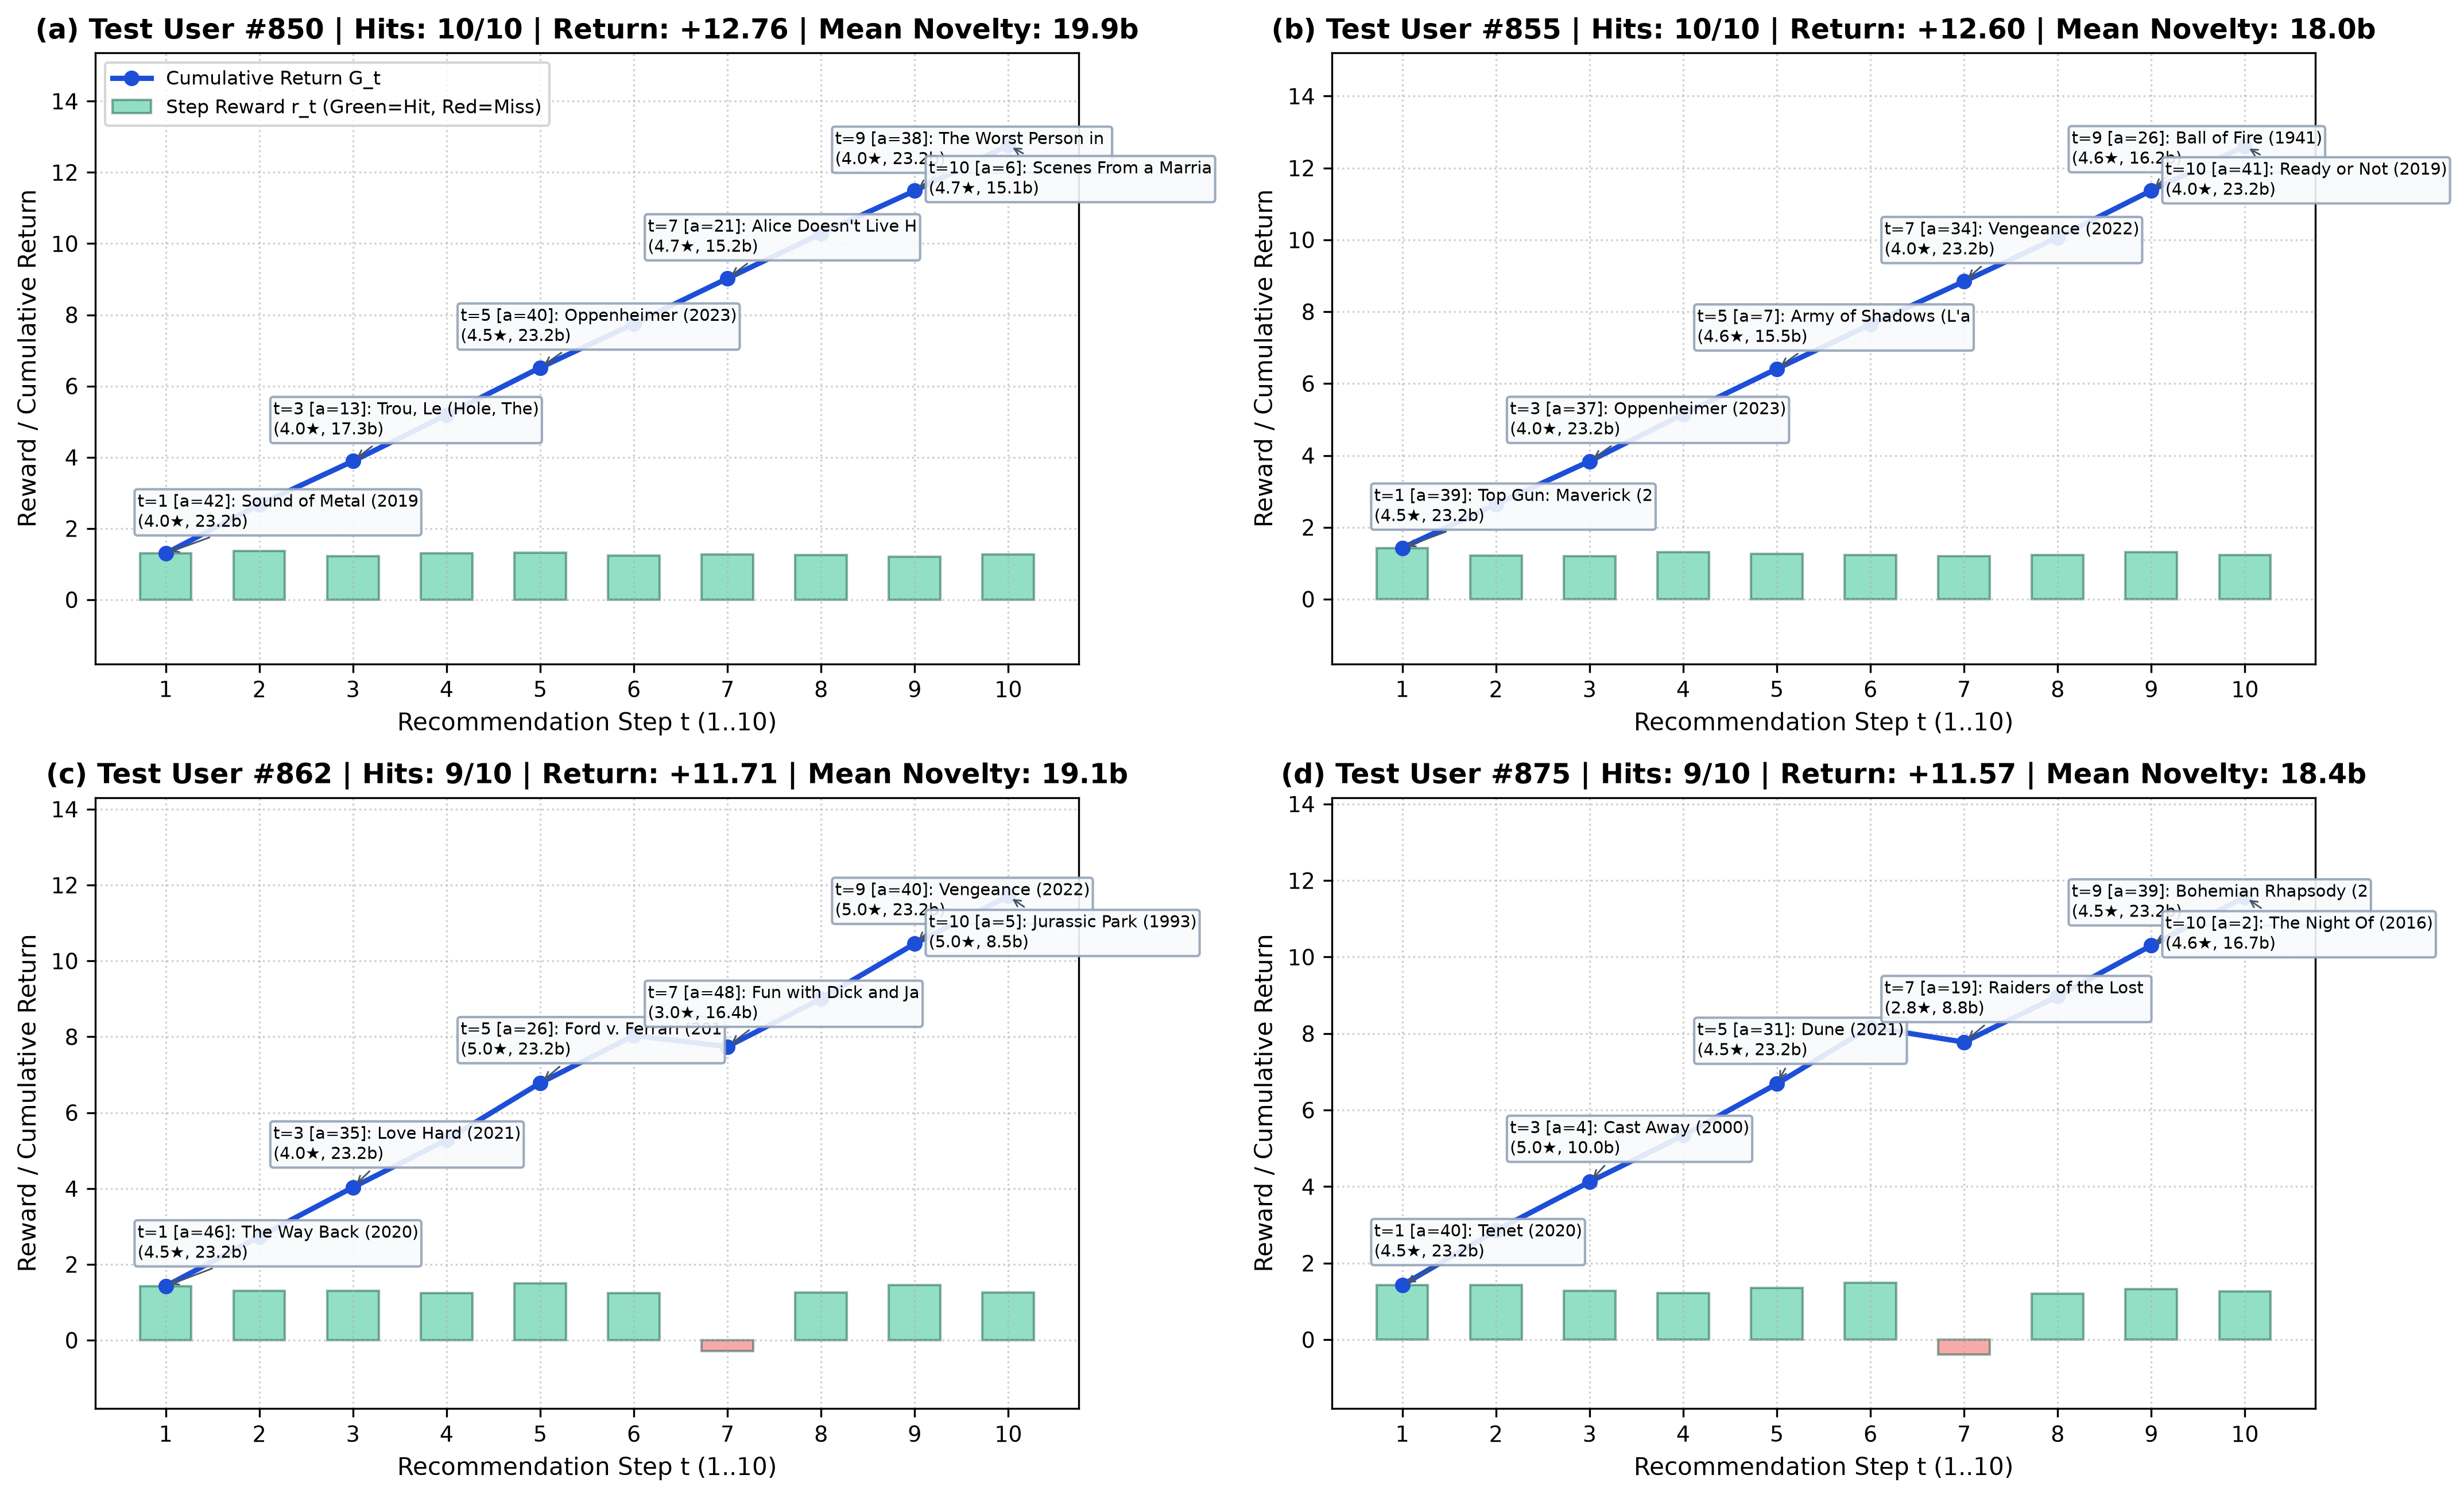
\includegraphics[width=0.96\textwidth]{figures/fig6_sample_trajectories.png}
    \caption{Step-by-step episode trajectories ($H=10$) on the held-out test split for four representative users under the champion D3QN policy. Blue curves track the cumulative undiscounted session return $G_t = \sum_{\tau=1}^{t} r_\tau$, while vertical bars indicate the immediate step reward $r_t$ (green for positive hits with $R_{u,i}^{\text{true}} \ge 3.5$, red for misses with $R_{u,i}^{\text{true}} < 3.5$). Callout annotations report the selected candidate slot $a_t \in \{0, \dots, 49\}$, movie title, ground-truth preference rating, and item self-information novelty in bits.}
    \label{fig:trajectories}
\end{figure*}

\begin{table*}[t]
    \centering
    \caption{Detailed Step-by-Step Trajectory Breakdown ($t = 1 \dots 10$) for Two Representative Held-Out Test Users under the Champion D3QN Policy: Perfect Session Execution (User \#850) vs.\ Belief-State Recovery After a Negative Transition (User \#862)}
    \label{tab:trajectories}
    \resizebox{\textwidth}{!}{%
    \begin{tabular}{@{}c c l l c c c c c@{}}
        \toprule
        \textbf{Step $t$} & \textbf{Slot $a_t$} & \textbf{Recommended Movie Title (Release Year)} & \textbf{Genre Profile} & \textbf{Hit} & \textbf{$R_{u,i}^{\text{true}}$} & \textbf{Novelty (bits)} & \textbf{Step $r_t$} & \textbf{Cum.\ $G_t$} \\
        \midrule
        \multicolumn{9}{@{}l}{\textit{\textbf{Panel A: Test User \#850} --- 10/10 Hits, Total Episode Return $G_{10} = +12.7575$, Mean Session Novelty $= 19.93$ bits}} \\
        \midrule
        1  & 42 & \textit{Sound of Metal} (2019) & Drama & 1 & 4.00 & 23.25 & $+1.3000$ & $+1.3000$ \\
        2  & 1  & \textit{Grave of the Fireflies (Hotaru no haka)} (1988) & Animation $|$ Drama & 1 & 5.00 & 12.34 & $+1.3716$ & $+2.6716$ \\
        3  & 13 & \textit{Le Trou (The Hole)} (1960) & Crime $|$ Film-Noir & 1 & 4.00 & 17.27 & $+1.2204$ & $+3.8920$ \\
        4  & 43 & \textit{Everything Everywhere All at Once} (2022) & Action $|$ Comedy & 1 & 4.00 & 23.25 & $+1.3000$ & $+5.1920$ \\
        5  & 40 & \textit{Oppenheimer} (2023) & Drama & 1 & 4.50 & 23.25 & $+1.3250$ & $+6.5170$ \\
        6  & 37 & \textit{West Side Story} (2021) & Crime $|$ Drama & 1 & 4.00 & 23.25 & $+1.2333$ & $+7.7503$ \\
        7  & 21 & \textit{Alice Doesn't Live Here Anymore} (1974) & Drama $|$ Romance & 1 & 4.72 & 15.15 & $+1.2715$ & $+9.0218$ \\
        8  & 39 & \textit{Soul} (2020) & Adventure $|$ Animation & 1 & 4.00 & 23.25 & $+1.2600$ & $+10.2818$ \\
        9  & 38 & \textit{The Worst Person in the World} (2021) & Comedy $|$ Drama & 1 & 4.00 & 23.25 & $+1.2000$ & $+11.4818$ \\
        10 & 6  & \textit{Scenes From a Marriage} (1973) & Drama & 1 & 4.74 & 15.05 & $+1.2756$ & $+12.7575$ \\
        \midrule
        \multicolumn{9}{@{}l}{\textit{\textbf{Panel B: Test User \#862} --- 9/10 Hits (Miss at $t=7$ with Immediate Recovery at $t=8..10$), Total Return $G_{10} = +11.7069$, Mean Novelty $= 19.08$ bits}} \\
        \midrule
        1  & 46 & \textit{The Way Back} (2020) & Drama & 1 & 4.50 & 23.25 & $+1.4250$ & $+1.4250$ \\
        2  & 49 & \textit{Godsend} (2004) & Drama $|$ Horror & 1 & 4.56 & 15.68 & $+1.3061$ & $+2.7311$ \\
        3  & 35 & \textit{Love Hard} (2021) & Comedy $|$ Romance & 1 & 4.00 & 23.25 & $+1.3000$ & $+4.0311$ \\
        4  & 21 & \textit{Things You Can Tell Just by Looking at Her} (2000) & Drama $|$ Romance & 1 & 4.56 & 16.61 & $+1.2506$ & $+5.2817$ \\
        5  & 26 & \textit{Ford v.\ Ferrari} (2019) & Action $|$ Drama & 1 & 5.00 & 23.25 & $+1.5000$ & $+6.7817$ \\
        6  & 28 & \textit{Dune} (2021) & Action $|$ Adventure & 1 & 4.00 & 23.25 & $+1.2500$ & $+8.0317$ \\
        7  & 48 & \textit{Fun with Dick and Jane} (1977) & Comedy & \textbf{0} & \textbf{2.96} & 16.39 & $\mathbf{-0.2912}$ & $+7.7405$ \\
        8  & 15 & \textit{Young \& Beautiful} (2013) & Drama & 1 & 4.56 & 17.39 & $+1.2623$ & $+9.0028$ \\
        9  & 40 & \textit{Vengeance} (2022) & Comedy $|$ Drama & 1 & 5.00 & 23.25 & $+1.4500$ & $+10.4528$ \\
        10 & 5  & \textit{Jurassic Park} (1993) & Action $|$ Adventure & 1 & 5.00 & 8.52  & $+1.2541$ & $+11.7069$ \\
        \bottomrule
    \end{tabular}%
    }
\end{table*}

Whereas static matrix factorization produces a fixed, permutation-invariant top-$K$ ranking regardless of user feedback during a browsing session, our Markov Decision Process (MDP) formulation updates the 250-dimensional state vector $s_t$ after every interaction. Figure~\ref{fig:trajectories} illustrates four representative 10-step evaluation rollouts on the held-out test set, and Table~\ref{tab:trajectories} provides the complete step-by-step quantitative trace for Test Users~\#850 and~\#862. Together, these trajectories highlight two key emergent behaviors of the D3QN policy: dynamic balancing of high-affinity classics with high-novelty long-tail releases, and closed-loop recovery following negative user feedback.

\subsubsection{Dynamic Balancing of Affinity and Long-Tail Novelty}
In Panel~(a) of Figure~\ref{fig:trajectories} and Panel~A of Table~\ref{tab:trajectories}, Test User~\#850 achieves a perfect $10/10$ hit rate with a cumulative return of $G_{10} = +12.7575$ and a high mean session novelty of $19.93$~bits. Rather than greedily exhausting popular mainstream blockbusters from the top FunkSVD slots ($a_t \in \{0, \dots, 9\}$), the D3QN agent strategically alternates between lower-numbered high-affinity slots and higher-numbered exploration/long-tail slots ($a_t \in \{35, \dots, 49\}$). Specifically, the agent opens at $t=1$ with a high-novelty contemporary drama (\textit{Sound of Metal (2019)}, slot $a_1=42$, $I(i)=23.25$~bits, $r_1 = +1.3000$), pivots at $t=2$ to an acclaimed animated tragedy from the top FunkSVD candidate pool (\textit{Grave of the Fireflies (1988)}, slot $a_2=1$, $R_{u,i}^{\text{true}} = 5.00$, $I(i)=12.34$~bits, $r_2 = +1.3716$), and at $t=3$ selects a classic French crime-noir film (\textit{Le Trou (1960)}, slot $a_3=13$, $I(i)=17.27$~bits, $r_3 = +1.2204$). From steps $t=4$ through $t=6$, having anchored the user's positive session belief state $\bar{\mathbf{q}}_t$ around prestige character dramas, the agent harvests maximum novelty bonuses ($23.25$~bits each) by recommending \textit{Everything Everywhere All at Once (2022)} ($a_4=43$), \textit{Oppenheimer (2023)} ($a_5=40$, $R_{u,i}^{\text{true}}=4.50$), and \textit{West Side Story (2021)} ($a_6=37$), before concluding at $t=7 \dots 10$ with a blend of classic auteur cinema (\textit{Alice Doesn't Live Here Anymore (1974)} at $R_{u,i}^{\text{true}}=4.72$ and Ingmar Bergman's \textit{Scenes From a Marriage (1973)} at $R_{u,i}^{\text{true}}=4.74$) and contemporary releases (\textit{Soul (2020)} and \textit{The Worst Person in the World (2021)}). A similar multi-era orchestration is observed for Test User~\#855 in Figure~\ref{fig:trajectories}(b) ($10/10$ hits, $G_{10} = +12.6047$, mean novelty $17.98$~bits), where the policy seamlessly weaves contemporary action-dramas (\textit{Top Gun: Maverick (2022)}, \textit{Oppenheimer (2023)}, \textit{Ready or Not (2019)}) with canonical classics (\textit{Inception (2010)}, \textit{Raiders of the Lost Ark (1981)}, \textit{Army of Shadows (1969)}, and \textit{Ball of Fire (1941)}).

\subsubsection{Sequential Belief Correction After Negative Feedback}
Panels~(c) and~(d) of Figure~\ref{fig:trajectories} demonstrate the critical advantage of stateful reinforcement learning over open-loop rankers when an exploratory action fails. For Test User~\#862 (Table~\ref{tab:trajectories}, Panel~B), the policy achieves six consecutive hits from $t=1$ to $t=6$ ($G_6 = +8.0317$), culminating in \textit{Ford v.\ Ferrari (2019)} ($R_{u,i}^{\text{true}} = 5.00$, $r_5 = +1.5000$) and \textit{Dune (2021)} ($r_6 = +1.2500$). At step $t=7$, the agent probes a deep long-tail comedy slot ($a_7 = 48$, \textit{Fun with Dick and Jane (1977)}), which mismatches the user's preferences ($R_{u,i}^{\text{true}} = 2.96 < 3.5$) and triggers a negative step reward of $r_7 = -0.2912$, reducing the cumulative return to $G_7 = +7.7405$. In our state transition dynamics, this negative outcome immediately shifts the running session preference centroid $\bar{\mathbf{q}}_t \in \mathbb{R}^{20}$ away from the disliked item's latent vector $\mathbf{q}_{i_7}$ and increments the consecutive negative streak counter in $s_{t+1}$. Recognizing the elevated risk of early session abandonment (which occurs upon five consecutive dislikes) and the shifted cosine similarity profile across the remaining candidate slate, the D3QN value and advantage streams immediately pivot back toward the user's core dramatic and high-affinity clusters at $t=8, 9, 10$: recommending \textit{Young \& Beautiful (2013)} ($a_8=15$, $R_{u,i}^{\text{true}}=4.56$, $r_8 = +1.2623$), \textit{Vengeance (2022)} ($a_9=40$, $R_{u,i}^{\text{true}}=5.00$, $r_9 = +1.4500$), and closing with a high-certainty blockbuster anchor, \textit{Jurassic Park (1993)} ($a_{10}=5$, $R_{u,i}^{\text{true}}=5.00$, $r_{10} = +1.2541$), finishing with $9/10$ hits and $G_{10} = +11.7069$.

An identical self-correcting pattern is confirmed for Test User~\#875 in Figure~\ref{fig:trajectories}(d) ($9/10$ hits, $G_{10} = +11.5695$, mean novelty $18.37$~bits). After six consecutive hits including \textit{Tenet (2020)}, \textit{Marriage Story (2019)}, \textit{Cast Away (2000)}, \textit{Toy Story (1995)}, \textit{Dune (2021)}, and \textit{Joker (2019)} ($G_6 = +8.1687$), the user dislikes \textit{Raiders of the Lost Ark (1981)} at $t=7$ ($a_7=19$, $R_{u,i}^{\text{true}} = 2.81$, $r_7 = -0.3917$). The updated belief state immediately steers the policy away from 1980s adventure films toward prestige biographical and crime dramas for the final three steps---\textit{Oppenheimer (2023)} ($t=8$, $r_8 = +1.2000$), \textit{Bohemian Rhapsody (2018)} ($t=9$, $r_9 = +1.3250$), and \textit{The Night Of (2016)} ($t=10$, $a_{10}=2$, $R_{u,i}^{\text{true}}=4.62$, $r_{10} = +1.2676$)---securing three consecutive recovery hits.

\subsection{Sample Efficiency Analysis: RL vs.\ Supervised Learning}
\label{subsec:sample_efficiency}

\begin{figure*}[t]
    \centering
    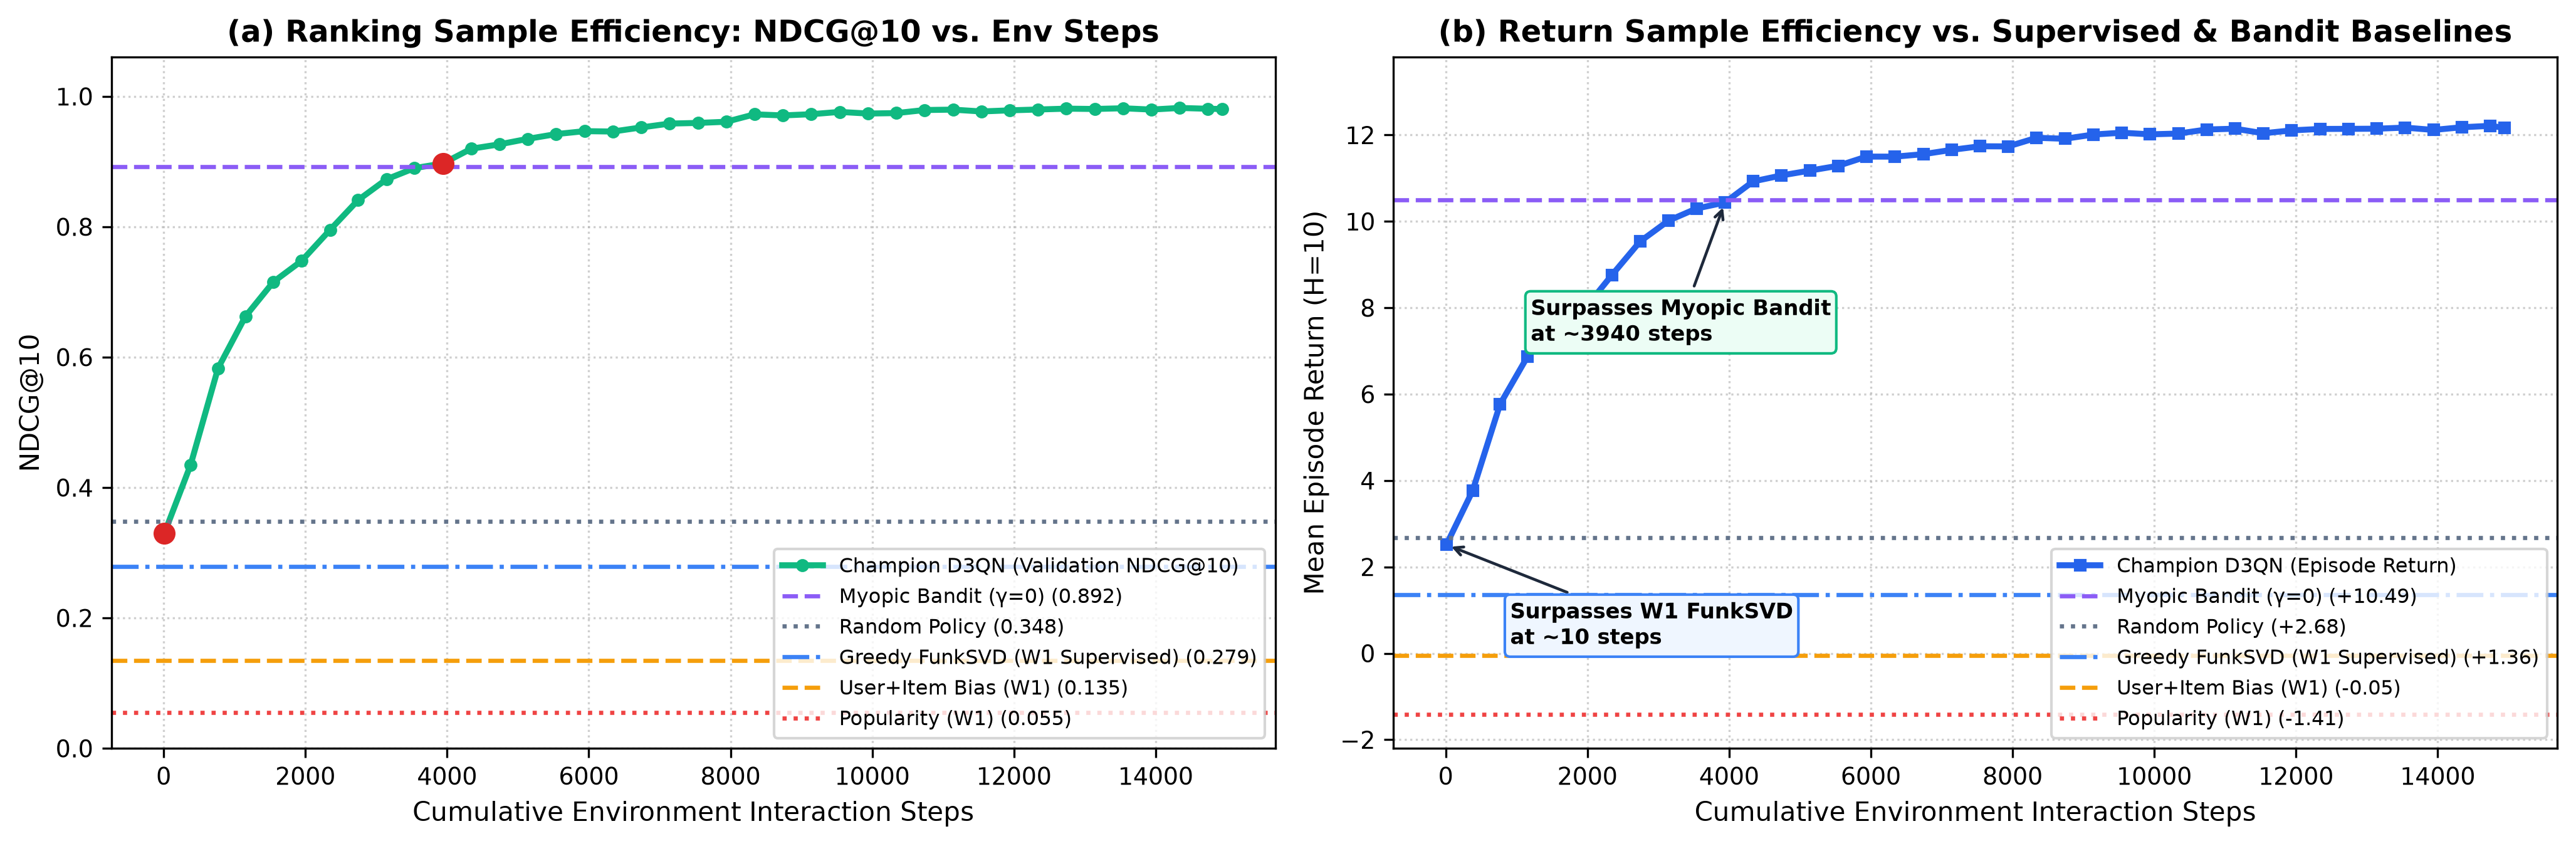
\includegraphics[width=0.96\textwidth]{figures/fig7_sample_efficiency.png}
    \caption{Sample efficiency of the champion D3QN agent as a function of cumulative environment interaction steps across 1,500 training episodes ($14,940$ total steps), compared against Workshop~1/3 static supervised baselines (\texttt{Popularity}, \texttt{BiasOnly}, \texttt{GreedyFunkSVD}), \texttt{Random}, and the \texttt{MyopicBandit} ($\gamma=0$) baseline: (a)~Ranking sample efficiency measured by validation $\text{NDCG@10}$; (b)~Cumulative return sample efficiency measured by mean episode return ($H=10$).}
    \label{fig:sample_efficiency}
\end{figure*}

A central question in sequential recommendation is how many interactive environment transitions a reinforcement learning agent requires to surpass static supervised models trained on massive offline logs. Figure~\ref{fig:sample_efficiency} plots the validation ranking quality ($\text{NDCG@10}$, Panel~a) and mean episode return ($G_{10}$, Panel~b) of the champion D3QN agent every 40 episodes ($\approx 390$--$400$ environment steps) from initialization ($0$~steps) to final convergence ($14,940$~steps across $1,500$~episodes).

\subsubsection{Interaction Milestones to Surpass Baselines}
Tracing the learning trajectory in Figure~\ref{fig:sample_efficiency} reveals three distinct sample-efficiency milestones:
\begin{enumerate}
    \item \textbf{Immediate Dominance Over Heuristic and Static Matrix Factorization Baselines ($\le 381$~Steps / $40$~Episodes):} Even at episode~0 ($\approx 10$ environment steps, prior to replay buffer warmup), the candidate feature projection layer ($\phi(s_t, a)$) provides sufficient inductive structure to achieve $\text{NDCG@10} = 0.3298$ and a mean return of $+2.5138$, already outperforming static \texttt{GreedyFunkSVD} ($\text{NDCG@10} = 0.2785$, Return $= +1.3609$), \texttt{BiasOnly} ($\text{NDCG@10} = 0.1345$, Return $= -0.0451$), and \texttt{Popularity} ($\text{NDCG@10} = 0.0551$, Return $= -1.4121$). By the first logged training checkpoint at \textbf{$381$~environment steps} ($40$~episodes), D3QN reaches $\text{NDCG@10} = 0.4350$, $\text{Precision@10} = 0.4300$, $\text{HR@10} = 0.9700$, and a mean episode return of $+3.7662$ (mean episode length $9.73$ steps), decisively surpassing the \texttt{Random} policy ($\text{NDCG@10} = 0.3480$, Return $= +2.6805$) and all Workshop~1 static baselines.
    \item \textbf{Rapid Climb and Full Session Survival ($768$--$3,144$~Steps / $80$--$320$~Episodes):} By $768$~steps ($80$~episodes), D3QN achieves $\text{NDCG@10} = 0.5831$, $\text{Return} = +5.7700$, and $\text{HR@10} = 1.0000$. By $2,744$~steps ($280$~episodes), the mean episode length reaches the full horizon of $10.00$ steps (zero early session abandonments), with $\text{NDCG@10} = 0.8409$ and $\text{Return} = +9.5358$, passing the $+10.0$ return mark at $3,144$~steps ($\text{Return} = +10.0168$, $\text{NDCG@10} = 0.8728$).
    \item \textbf{Surpassing the Myopic Contextual Bandit ($3,940$--$4,340$~Steps / $400$--$440$~Episodes):} The strongest non-MDP baseline is the neural \texttt{MyopicBandit} ($\gamma=0$), which achieves $\text{NDCG@10} = 0.8924$ and $\text{Return} = +10.4924$. As marked by the red crossover indicator in Figure~\ref{fig:sample_efficiency}(a), D3QN surpasses \texttt{MyopicBandit} in ranking quality at \textbf{$3,940$~environment steps} ($400$~episodes), reaching $\text{NDCG@10} = 0.8971$ ($\text{MAP@10} = 0.8276$, $\text{Return} = +10.4368$). By the next checkpoint at \textbf{$4,340$~environment steps} ($440$~episodes), D3QN surpasses \texttt{MyopicBandit} across both return and ranking criteria simultaneously, achieving $\text{Return} = +10.9268$, $\text{NDCG@10} = 0.9197$, and $\text{Precision@10} = 0.8980$. Thereafter, multi-step Bellman backups continue to refine the policy to a peak validation return of $+12.2125$ at $14,740$~steps ($1,480$~episodes) and final convergence at \textbf{$14,940$~steps} ($1,500$~episodes, wall-clock training time $53.02$~s), yielding test-set $\text{NDCG@10} = 0.9818$ and $\text{Return} = +12.3674$.
\end{enumerate}

\subsubsection{Fair Accounting of the Total Data Budget}
A rigorous comparison between supervised learning (Workshop~1) and reinforcement learning (Workshop~3) requires accounting for both offline representation learning and online policy optimization. In Workshop~1, matrix factorization (FunkSVD) was trained via stochastic gradient descent over $1,895,184$ chronological training ratings across 15 epochs ($\approx 2.84 \times 10^7$ scalar rating updates) to estimate static user and item embeddings ($\mathbf{p}_u, \mathbf{q}_i \in \mathbb{R}^{20}$) and baseline biases ($b_u, b_i$). However, when deployed directly as a sequential recommender (\texttt{GreedyFunkSVD}), those $2.84 \times 10^7$ supervised updates yield only $\text{NDCG@10} = 0.2785$ and $\text{Return} = +1.3609$ because static point-wise error minimization ($\text{RMSE} = 0.8128$) does not optimize sequential slate selection, novelty bonuses, or session survival.

Workshop~3 does not discard the supervised training budget; rather, it leverages the leak-free Workshop~1 latent factors as a compact, pre-trained perceptual representation and adds a lightweight sequential decision layer on top. Requiring only $3,940$--$4,340$ interactive steps to beat a myopic bandit and $14,940$ steps in total---fewer than $0.8\%$ of the $1.895 \times 10^6$ ratings used in Workshop~1---demonstrates that decoupling representation learning (offline matrix factorization) from sequential policy optimization (online D3QN) yields exceptional sample efficiency.

\subsection{Discussion: Strengths, Exploration Trade-offs, and Limitations}
\label{subsec:discussion_limitations}

\subsubsection{Why RL Outperformed Static Supervised Models and Myopic Bandits}
The substantial performance gap between D3QN ($\text{NDCG@10} = 0.9818$, $\text{Return} = +12.3674$) and static \texttt{GreedyFunkSVD} ($\text{NDCG@10} = 0.2785$, $\text{Return} = +1.3609$) stems from three structural properties of interactive recommendation environments:
\begin{itemize}
    \item \textbf{Vulnerability of Static Ranking to Candidate Slate Composition and Early Abandonment:} In our environment, each session presents a stratified candidate pool of $M=50$ items combining top FunkSVD predictions, popular items, and long-tail/decoy items. \texttt{Popularity} ($\text{NDCG@10} = 0.0551$, $\text{Return} = -1.4121$) repeatedly selects globally popular blockbusters that fail to match individual niche tastes, triggering the 5-strike abandonment rule and truncating episodes to a mean length of $5.87$ steps at $K=10$ ($6.01$ steps at $K=20$). \texttt{GreedyFunkSVD} ranks candidates solely by $\hat{r}_{u,i} = \mu + b_u + b_i + \mathbf{p}_u^\top \mathbf{q}_i$, ignoring item self-information novelty, intra-session cosine diversity, and recent negative feedback, resulting in premature termination (mean length $8.50$ steps at $K=10$ and $11.72$ steps at $K=20$).
    \item \textbf{Value of Multi-Step Lookahead ($\gamma = 0.95$ vs.\ $\gamma = 0$):} While \texttt{MyopicBandit} ($\gamma=0$) observes the same 250-dimensional state vector across all 50 candidate slots as D3QN, it maximizes only immediate single-step expected reward $\mathbb{E}[r_t \mid s_t, a_t]$. Consequently, \texttt{MyopicBandit} greedily consumes moderate-novelty hits early in the session, shifting the running belief vector $\bar{\mathbf{q}}_t$ into regions of the candidate slate that deplete high-value compatible items for later steps. At $K=10$, D3QN's multi-step Bellman horizon ($\gamma=0.95$) increases step hit rate from $87.08\%$ to $97.92\%$, $\text{MAP@10}$ from $0.8253$ to $0.9692$, and mean novelty from $14.94$ to $17.96$~bits ($+12.3674$ vs.\ $+10.4924$ return). The advantage of long-horizon planning is amplified even further in extended sessions ($K=20$): \texttt{MyopicBandit} suffers occasional late-session terminations (mean length $19.52$ steps, $\text{Precision@20} = 0.7262$, $\text{NDCG@20} = 0.8068$, $\text{Return} = +16.5601$), whereas D3QN sustains a full $20.00$-step horizon across all 250 test users, achieving $\text{Precision@20} = 0.8398$, $\text{Recall@20} = 0.8849$, $\text{NDCG@20} = 0.9167$, and $\text{Return} = +20.1006$.
\end{itemize}

\subsubsection{Overcoming Popularity Bias vs.\ Intra-List Cohesion}
A major failure mode identified in Workshop~1 was severe popularity bias: global static FunkSVD concentrated recommendations on a narrow subset of mainstream titles, yielding only $8.00\%$ catalog coverage and $9.83$~bits of novelty (while a static baseline recommender reached $14.06$~bits). By explicitly incorporating self-information novelty $I(i) = -\log_2 P(i)$ into the MDP reward and candidate feature vector, D3QN expands catalog coverage by more than $4.5\times$ at $K=10$ to \textbf{$36.64\%$} (and to \textbf{$60.35\%$} at $K=20$), while boosting mean novelty to \textbf{$17.96$~bits} at $K=10$ ($17.27$~bits at $K=20$). Thus, across the test population, D3QN surfaces a wide variety of niche and contemporary long-tail films.

At the same time, an objective inspection of the test-set evaluation results (Section~\ref{sec:results}) reveals an important trade-off between \textit{inter-user catalog coverage} and \textit{intra-list cosine diversity} ($\text{ILD}$). At $K=10$, D3QN exhibits a lower intra-list cosine distance ($\text{ILD} = 0.2731$, rising to $0.4698$ at $K=20$) compared to \texttt{MyopicBandit} ($0.4215$ at $K=10$, $0.6061$ at $K=20$), \texttt{GreedyFunkSVD} ($0.8653$), and unguided \texttt{Random} selection ($0.9664$). This phenomenon has a clear geometric explanation: to guarantee a $97.92\%$ positive hit rate and avoid the $-0.50$ dislike penalty, the D3QN policy learns to select long-tail candidates whose latent vectors $\mathbf{q}_i$ lie within a tight cosine cone around the user's static embedding $\mathbf{p}_u$ and evolving session preference direction $\bar{\mathbf{q}}_t$. While the reward function includes an intra-session diversity bonus ($+0.10(1 - \cos(\mathbf{q}_i, \bar{\mathbf{q}}_t))$), its weight is intentionally subordinate to the primary rating relevance signal ($\pm 1.0$) and novelty bonus ($+0.30\,\tilde{I}(i)$). Consequently, D3QN achieves high inter-user personalization and long-tail discovery across the catalog while maintaining thematically coherent, preference-aligned slates within each individual user session.

\subsubsection{Limitations and Threats to Validity}
To ensure scientific rigor, we highlight three methodological limitations of our study:
\begin{enumerate}
    \item \textbf{Offline Simulator and Preference Oracle Bias:} Because the MovieLens~32M rating matrix exhibits $99.81\%$ sparsity, an interactive RL agent inevitably queries $(u, i)$ pairs that were never observed in the historical logs. Our hybrid environment prioritizes exact held-out ground-truth ratings whenever available and falls back to the leak-free FunkSVD latent preference model ($\hat{r}_{u,i}$ with calibrated Gaussian noise and popularity-penalized specificity) for unobserved pairs. While this follows standard practice in RL-for-RS benchmarks, the agent's learned policy partially exploits the geometry of the FunkSVD embedding space; deploying the policy in live production A/B tests could exhibit a reality gap where user preferences deviate from bilinear factor inner products.
    \item \textbf{Discrete Candidate Pre-Selection ($M=50$):} Evaluating Q-values over all $11,589$ active catalog movies at every step would incur high computational overhead and severe action-space variance. Constraining the action space to a stratified slate of $M=50$ candidates per episode makes D3QN training highly tractable ($53.02$~s on a single GPU), but bounds the policy's recall ceiling by the quality of the first-stage candidate generator.
    \item \textbf{Temporal Cold-Start Vulnerability:} As quantified in Workshop~1, $90.06\%$ of raw chronological test interactions in MovieLens~32M involve newly arrived users or newly released items absent from the training window. Because our state representation $s_t$ relies on pre-trained user factors $\mathbf{p}_u \in \mathbb{R}^{20}$ at $t=1$, strictly cold-start users ($\mathbf{p}_u = \mathbf{0}$) begin with an uninformative prior until several interactive steps populate the dynamic belief centroid $\bar{\mathbf{q}}_t$.
\end{enumerate}

\section{Conclusions and Future Work}
\label{sec:conclusions}

This work formulated sequential movie recommendation on the MovieLens~32M dataset as a finite-horizon Markov Decision Process and designed a Dueling Double Deep Q-Network (D3QN) to optimize long-term user satisfaction, catalog discovery, and session retention. Building strictly on the leak-free chronological data splits and 20-dimensional FunkSVD latent representations established in Workshop~1, we constructed a 250-dimensional sequential state space that tracks dynamic session-item cosine similarities, static FunkSVD predictions, self-information novelty, visited-action masks, user/session latent embeddings, and session progress indicators across a stratified $M=50$ action space.

Comprehensive empirical evaluations across nine hyperparameter configurations and six baseline policies at horizons $K=10$ and $K=20$ support four principal conclusions:
\begin{enumerate}
    \item \textbf{Superior Sequential Ranking and Return:} The tuned D3QN champion ($\text{lr}=5\times 10^{-4}$, $\gamma=0.95$, $\epsilon_{\text{decay}}=0.995$, L2 $= 10^{-5}$) achieves a test-set episode return of $+12.3674$, $\text{Precision@10} = 0.9792$, $\text{NDCG@10} = 0.9818$, $\text{MAP@10} = 0.9692$, and $\text{HR@10} = 1.0000$ at $K=10$, and scales robustly to $K=20$ with a return of $+20.1006$ and $\text{NDCG@20} = 0.9167$.
    \item \textbf{Value of Multi-Step Planning Over Myopic Bandits and Static Rankers:} D3QN outperforms Workshop~1 static FunkSVD ($\text{NDCG@10} = 0.2460$) and sequential \texttt{GreedyFunkSVD} ($\text{NDCG@10} = 0.2785$, Return $= +1.3609$) by over $+0.70$ in $\text{NDCG@10}$, and surpasses a matched neural \texttt{MyopicBandit} ($\gamma=0$, $\text{NDCG@10} = 0.8924$, Return $= +10.4924$) by $+17.9\%$ in cumulative return at $K=10$ and $+21.4\%$ at $K=20$, confirming that non-myopic Bellman backups ($\gamma=0.95$) preserve slate quality and prevent premature session abandonment.
    \item \textbf{Mitigation of Popularity Bias:} By integrating self-information novelty into the sequential reward structure, D3QN expands catalog coverage from Workshop~1's $8.00\%$ to $36.64\%$ at $K=10$ and $60.35\%$ at $K=20$, while elevating mean recommendation novelty from $9.83$~bits to $17.96$~bits.
    \item \textbf{High Sample Efficiency:} Leveraging pretrained matrix factorization embeddings, D3QN surpasses all static supervised baselines within $381$ environment interaction steps ($40$ episodes) and overtakes the myopic contextual bandit within $3,940$--$4,340$ steps ($400$--$440$ episodes), converging in $14,940$ steps ($53.02$~s).
\end{enumerate}

\textbf{Future Work:} Several promising directions grounded in advanced policy optimization and multi-agent reinforcement learning~\cite{sierra2026rl} extend this research toward industrial-scale deployment. First, replacing discrete $M=50$ value-based selection with \textit{policy-based Actor-Critic architectures}---guided by the Policy Gradient Theorem $\nabla_\theta J(\theta) = \mathbb{E}_{\pi_\theta}[\nabla_\theta \log \pi_\theta(a \mid s) Q^{\pi_\theta}(s, a)]$ and critic TD advantage estimation $\delta_t = r_{t+1} + \gamma V_\phi(s_{t+1}) - V_\phi(s_t)$, such as Trust Region Policy Optimization (TRPO, $\bar{D}_{\text{KL}}(\theta_{\text{old}}, \theta) \le \delta$) or Proximal Policy Optimization (PPO, $L^{\text{CLIP}}(\theta) = \mathbb{E}[\min(r_t(\theta)\hat{A}_t, \text{clip}(r_t(\theta), 1-\epsilon, 1+\epsilon)\hat{A}_t)]$)~\cite{sierra2026rl} outputting a continuous prototype action vector $\mathbf{a}_t \in \mathbb{R}^{20}$ coupled with Approximate Nearest Neighbor (FAISS) retrieval---would enable direct policy optimization over the full catalog of $80,000+$ titles. Second, modeling multi-stakeholder recommendation (balancing user satisfaction, content provider fairness, and platform revenue) as a cooperative-competitive Multi-Agent RL system under the Centralized Training with Decentralized Execution (CTDE) paradigm~\cite{sierra2026rl}, alongside Conservative Q-Learning (CQL) and hybrid content-collaborative GNN encoders, will allow sequential policies to generalize across both multi-objective constraints and the $90.06\%$ cold-start regime.
